\chapter{Testes e Resultados}
% Revisar

Os testes de infraestrutura desempenham um papel fundamental na garantia de que uma plataforma está pronta para ser utilizada em produção. Eles permitem verificar e validar aspectos cruciais da infraestrutura, como escalabilidade, tolerância a falhas, desempenho e segurança. Garantir que esses elementos estão funcionando conforme o esperado é essencial para proporcionar uma experiência de usuário satisfatória e para manter a integridade e disponibilidade da plataforma.

Neste capítulo, serão apresentados os testes realizados na plataforma Codeboard UERJ, com o objetivo de avaliar e validar sua escalabilidade, tolerância a falhas, desempenho e segurança. Os testes foram conduzidos em um ambiente de produção, visando simular situações reais de uso e identificar possíveis pontos de melhoria na infraestrutura.


\section{Distribuição de Carga}
% Revisar

Para avaliar a distribuição de carga em diferentes níveis da infraestrutura da plataforma Codeboard UERJ, foram realizadas modificações no código-fonte, permitindo a coleta de informações detalhadas sobre a máquina que processa cada requisição. Essas o identificador da instância EC2 na AWS e o identificador do processo (PID) responsável pelo processamento da requisição. Com esses dados, foi possível analisar como a carga está sendo distribuída entre diferentes regiões geográficas, servidores e processos.

\subsection{Balanceamento de Carga entre Regiões Geográficas} % TODO: FUDEU
% Revisar

Para analisar o balanceamento de carga entre diferentes regiões geográficas, utilizamos redes privadas virtuais (VPNs) para simular acessos à plataforma a partir de diversos locais ao redor do mundo. As VPNs são ferramentas que permitem alterar o endereço IP de origem de uma conexão, simulando o acesso de um usuário em uma região geográfica diferente da sua localização real.

Foram utilizadas cinco VPNs representando as regiões: Brasil, Estados Unidos, Europa, Ásia e Oceania. De cada uma dessas VPNs, realizamos 100 requisições à rota \texttt{/api/health}, e coletamos informações sobre o servidor que processou cada requisição e a latência observada. Os resultados estão apresentados na Tabela \ref{tab:geo-distribution}, e a Figura \ref{fig:geo-distribution} ilustra, em um mapa, o servidor designado para cada região geográfica.

% Atualmente usamos 5 VPNs: Brasil, Estados Unidos, Europa, Ásia e Oceania
% só existem dois servidores designados: Brasil e Estados Unidos
% TODO: Inserir dados
\begin{table}[H]
    \centering
    \caption{Resultados dos testes de distribuição de carga entre diferentes regiões geográficas}
    \label{tab:geo-distribution}
    \begin{tabular}{|l|l|l|}
        \hline
        \textbf{VPN}   & \textbf{Servidor Designado} & \textbf{Latência média} \\ \hline
        Brasil         & Brasil                      & 50 ms                   \\ \hline
        Estados Unidos & Estados Unidos              & 150 ms                  \\ \hline
        Europa         & Brasil                      & 200 ms                  \\ \hline
        Ásia           & Brasil                      & 300 ms                  \\ \hline
        Oceania        & Estados Unidos              & 400 ms                  \\ \hline
    \end{tabular}
\end{table}

% \begin{figure}[H]
%     \centering
%     \includegraphics[width=1\textwidth]{images/geo-distribution.png}
%     \caption{Distribuição de carga entre diferentes regiões geográficas}
%     \label{fig:geo-distribution}
% \end{figure}

Observando a Tabela \ref{tab:geo-distribution}, percebemos que o balanceamento de carga direciona as requisições para o servidor geograficamente mais próximo, sempre que possível. No caso do Brasil e dos Estados Unidos, as requisições são processadas pelos servidores correspondentes, reduzindo a latência e melhorando a experiência do usuário. Para as demais regiões, como Europa, Ásia e Oceania, as requisições foram direcionadas para o servidor dos Estados Unidos, o que resultou em latências maiores devido à distância geográfica.

Essa distribuição reflete a configuração atual da infraestrutura, que possui somente dois servidores, um no Brasil e outro nos Estados Unidos. A implementação de servidores adicionais em outras regiões poderia melhorar ainda mais a latência para usuários em locais distantes.

\subsection{Balanceamento de Carga entre Servidores}
% OK (revisar?)

Para avaliar o balanceamento de carga entre servidores dentro de uma mesma região, realizamos 5000 requisições à rota \texttt{/api/health} a partir da região geográfica do Brasil. Com as modificações feitas no código da plataforma, foi possível coletar as informações sobre qual servidor processou cada requisição.

Os resultados dos testes estão apresentados na Figura \ref{fig:reqs-per-instance} e na Figura \ref{fig:reqs-per-instance-over-time}, que mostram respectivamente a distribuição de carga entre diferentes servidores e a distribuição ao longo do tempo. Os dados coletados incluem a quantidade de requisições processadas por cada servidor e a identificação do servidor responsável pelo processamento.

\begin{figure}[H]
    \centering
    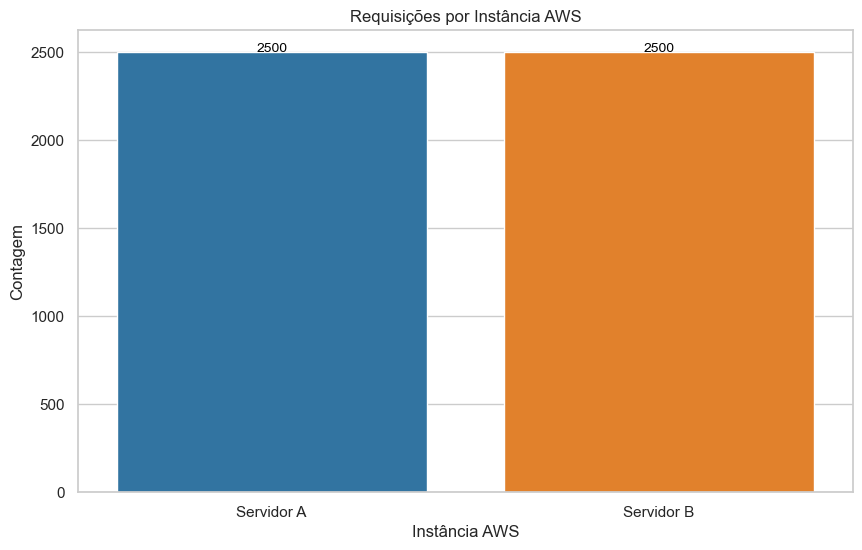
\includegraphics[width=1\textwidth]{assets/balance-test/reqs-per-instance.png}
    \caption{Distribuição de carga entre diferentes servidores}
    \label{fig:reqs-per-instance}
\end{figure}

\begin{figure}[H]
    \centering
    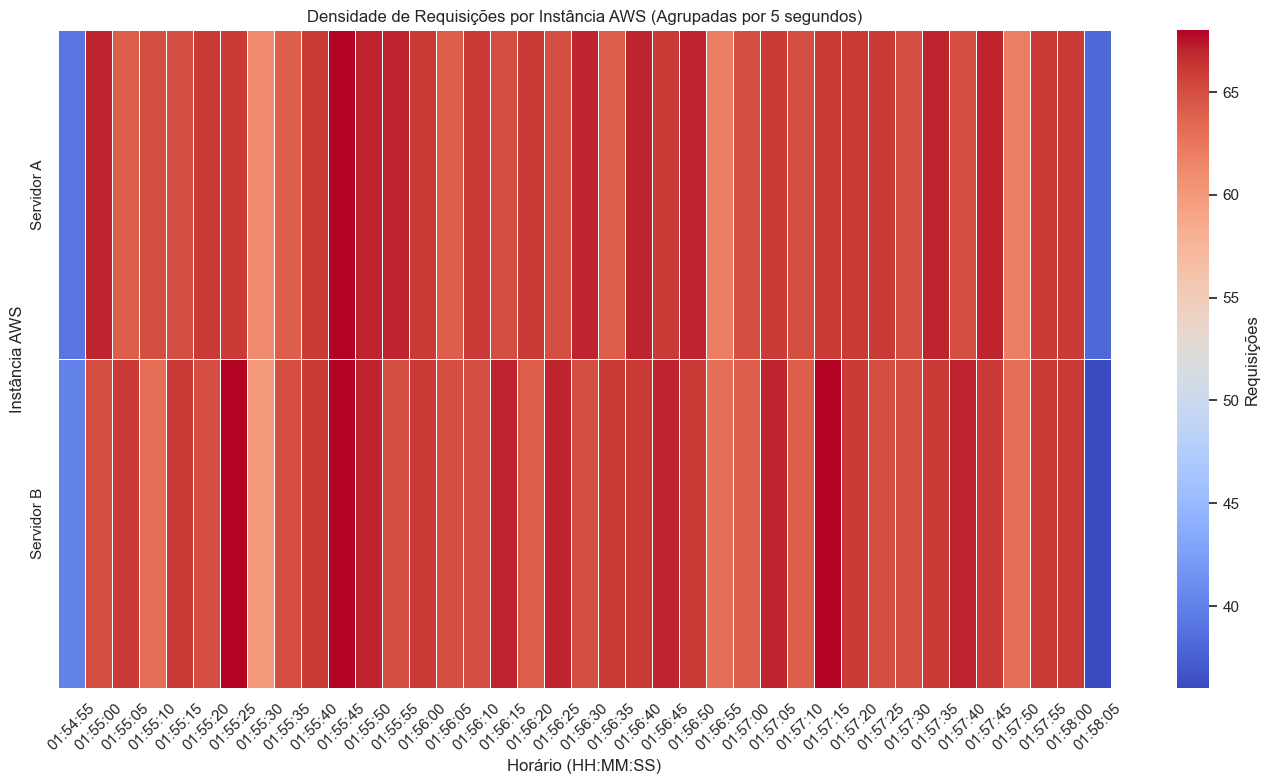
\includegraphics[width=1\textwidth]{assets/balance-test/reqs-per-instance-over-time.png}
    \caption{Distribuição de carga entre diferentes servidores ao longo do tempo}
    \label{fig:reqs-per-instance-over-time}
\end{figure}

Como pode ser observado na Figura \ref{fig:reqs-per-instance}, a distribuição de carga entre diferentes servidores foi realizada de forma eficiente, com metade das requisições sendo processadas por cada uma das instâncias disponíveis. O gráfico da Figura \ref{fig:reqs-per-instance-over-time} mostra que as requisições foram processadas de forma homogênea e alternada entre os dois servidores ao longo do tempo, validando a estratégia Round Robin utilizada para o balanceamento de carga entre diferentes servidores da infraestrutura.

Os dados indicam que o balanceador de carga distribuiu as requisições de forma equitativa entre os dois servidores disponíveis, validando a eficácia da estratégia de balanceamento utilizada. Essa distribuição contribuiu para uma utilização otimizada dos recursos presentes na infraestrutura e para a redução de possíveis gargalos de desempenho, evitando sobrecargas em um único servidor.

\subsection{Balanceamento de Carga entre Processos}
% OK (revisar!)

Para avaliar o balanceamento de carga entre processos dentro de um mesmo servidor, analisaremos novamente as 5000 requisições anteriormente realizadas para a rota \texttt{/api/health}. Desta vez, coletamos utilizaremos também o identificador do processo (PID) em nossa analise para identificar qual processo foi responsável pelo processamento de cada requisição.

Os resultados estão apresentados na Figura \ref{fig:reqs-per-pid}, que mostra a distribuição de carga entre diferentes processos, e na Figura \ref{fig:reqs-per-pid-over-time}, que mostra a distribuição ao longo do tempo. Os dados coletados incluem a quantidade de requisições processadas por cada processo, a identificação do servidor e do PID responsável pelo processamento.


\begin{figure}[H]
    \centering
    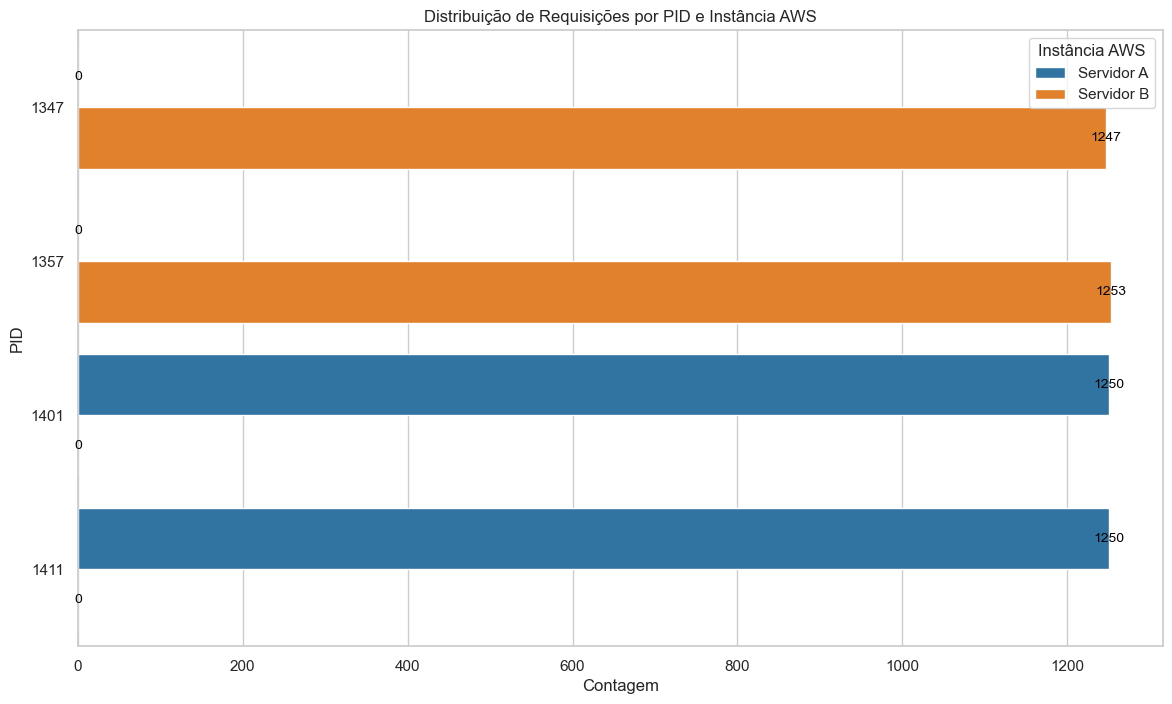
\includegraphics[width=1\textwidth]{assets/balance-test/reqs-per-pid.png}
    \caption{Distribuição de carga entre diferentes servidores}
    \label{fig:reqs-per-pid}
\end{figure}

\begin{figure}[H]
    \centering
    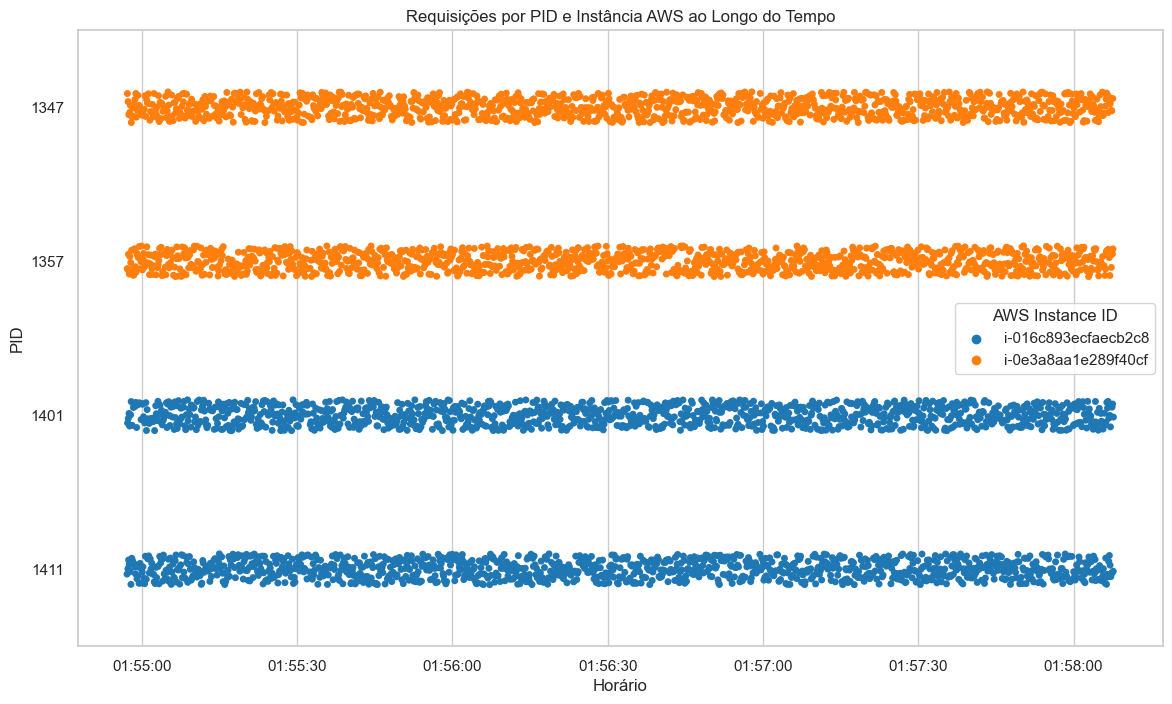
\includegraphics[width=1\textwidth]{assets/balance-test/reqs-per-pid-over-time.png}
    \caption{Distribuição de carga entre diferentes servidores ao longo do tempo}
    \label{fig:reqs-per-pid-over-time}
\end{figure}

Analisando os dados da Figura \ref{fig:reqs-per-pid}, observamos que as requisições foram distribuídas de forma quase que totalmente equilibra entre os processos disponíveis, com uma pequena diferença entre a quantidade de requisições processadas por cada um. O gráfico da Figura \ref{fig:reqs-per-pid-over-time} mostra que as requisições foram processadas de forma homogênea entre os diferentes processos ao longo do tempo, validando a estratégia de balanceamento de carga utilizada entre os núcleos de processamento dos servidores.

% TODO: Explicar o que é elasticidade no capítulo de conceitos
\section{Testes de Elasticidade}
% OK (revisar?)

Esta seção apresenta os testes de elasticidade realizados na plataforma Codeboard UERJ. Os testes foram realizados com o objetivo de validar a capacidade da infraestrutura de suportar um grande volume de usuários simultâneos, analisando o desempenho do servidor back-end em diferentes cenários de uso.


\subsection{Metodologia de Testes}

Os testes de elasticidade foram conduzidos utilizando a ferramenta Grafana K6, que permite simular um grande número de usuários acessando a plataforma simultaneamente. Configuramos a ferramenta para executar testes em etapas de carga progressiva, permitindo a medição de métricas como latência, taxa de erro e capacidade de resposta do sistema. Os testes foram divididos em três etapas principais:

\begin{enumerate}
    \item \textbf{Subida inicial:} Durante 10 minutos, o número de usuários simultâneos aumentou gradualmente até atingir 300.
    \item \textbf{Manutenção da carga:} O sistema manteve 300 usuários simultâneos por um período de 5 minutos.
    \item \textbf{Redução da carga:} A carga foi reduzida gradualmente para 0 ao longo de 5 minutos.
\end{enumerate}

Cada usuário simulado seguiu um fluxo típico de interação com a plataforma Codeboard UERJ, composto por cinco etapas principais: login, criação de sala, entrada na sala, codificação colaborativa e desconexão. Cada etapa envolveu a execução de requisições HTTP e comunicação via WebSocket, simulando o comportamento de um usuário real na plataforma.

\begin{enumerate}
    \item \textbf{Login:} Os usuários simulados iniciaram o fluxo realizando login na plataforma pela rota \texttt{/api/auth/login} utilizando credenciais válidas préviamente criadas no banco de dados. Após a autenticação, cada usuário recebeu um token JWT, essencial para acessar as funcionalidades subsequentes.
    \item \textbf{Criação de Sala:} Com o login concluído, os usuários criaram salas por meio da rota \texttt{/api/rooms}. Cada sala foi identificada por um nome único, e a API retornou um identificador correspondente à sala criada.
    \item \textbf{Entrada na Sala:} Após a criação, os usuários entraram nas salas utilizando a rota \texttt{/api/room/:roomId}. Eles buscaram informações da sala e se conectaram ao servidor WebSocket utilizando o token JWT e o identificador da sala. Durante essa etapa, enviaram as mensagens \texttt{room:join} e \texttt{board:join} para indicar que estavam prontos para iniciar a codificação colaborativa.
    \item \textbf{Escrita de Código:} Na etapa de codificação, os usuários interagiram via WebSocket, trocando mensagens de texto representativas de ações de escrita de código. Para simulação, cada usuário enviou 10 mensagens \texttt{board:write}, com intervalos de 3 segundos entre elas. Essas mensagens foram processadas pelo servidor e redistribuídas aos demais participantes da sala.
    \item \textbf{Desconexão:} Ao final da simulação, os usuários finalizaram a sessão de codificação enviando as mensagens \texttt{room:leave} e \texttt{board:leave}. Em seguida, desconectaram-se do servidor WebSocket. O servidor então gerou mensagens em fila para serem processadas posteriormente, salvando o código escrito no banco de dados e concluindo o ciclo de interação do usuário com a plataforma.
\end{enumerate}


\subsection{Resultados dos Testes}

Os resultados obtidos demonstram que a infraestrutura da plataforma Codeboard UERJ respondeu adequadamente às demandas simuladas, ajustando-se ao aumento e à redução do número de usuários sem apresentar falhas críticas. A seguir, detalhamos os principais resultados obtidos durante os testes:

\begin{figure}[H]
    \centering
    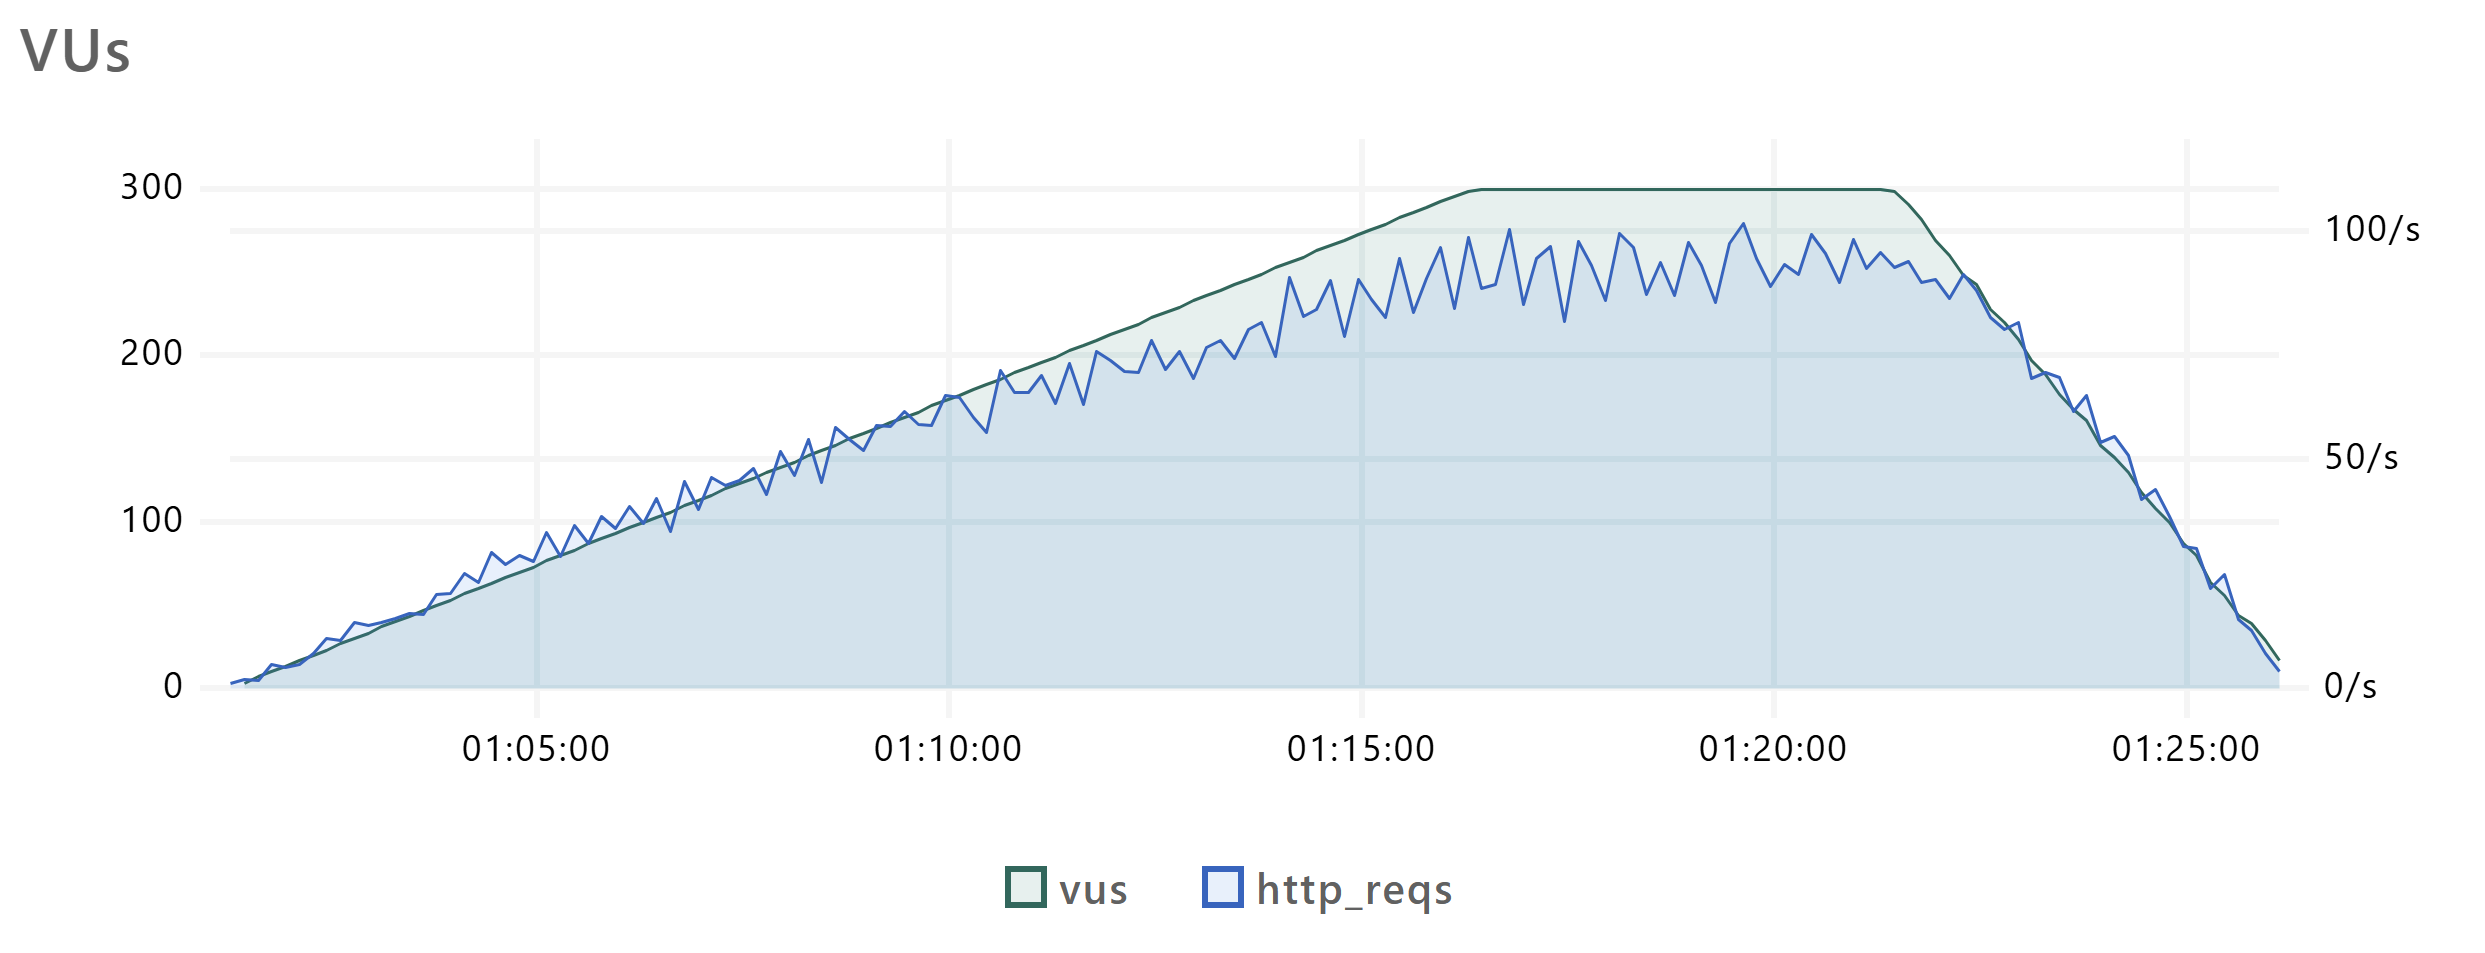
\includegraphics[width=1\textwidth]{assets/elasticity-test/vus-and-reqs.png}
    \caption{Número de usuários virtuais e taxa de requisições processadas por segundo ao longo do teste de elasticidade}
    \label{fig:elasticity-vus-and-reqs}
\end{figure}

Na Figura \ref{fig:elasticity-vus-and-reqs}, observa-se o comportamento do número de usuários simultâneos e da taxa de requisições por segundo processadas durante o teste. Conforme descrito na metodologia, o número de usuários aumentou gradualmente até 300, permaneceu constante por 5 minutos e foi reduzido a 0. A taxa de requisições processadas acompanhou o aumento e a redução do número de usuários, indicando que o sistema foi capaz de lidar com a carga de forma eficiente.

\begin{figure}[H]
    \centering
    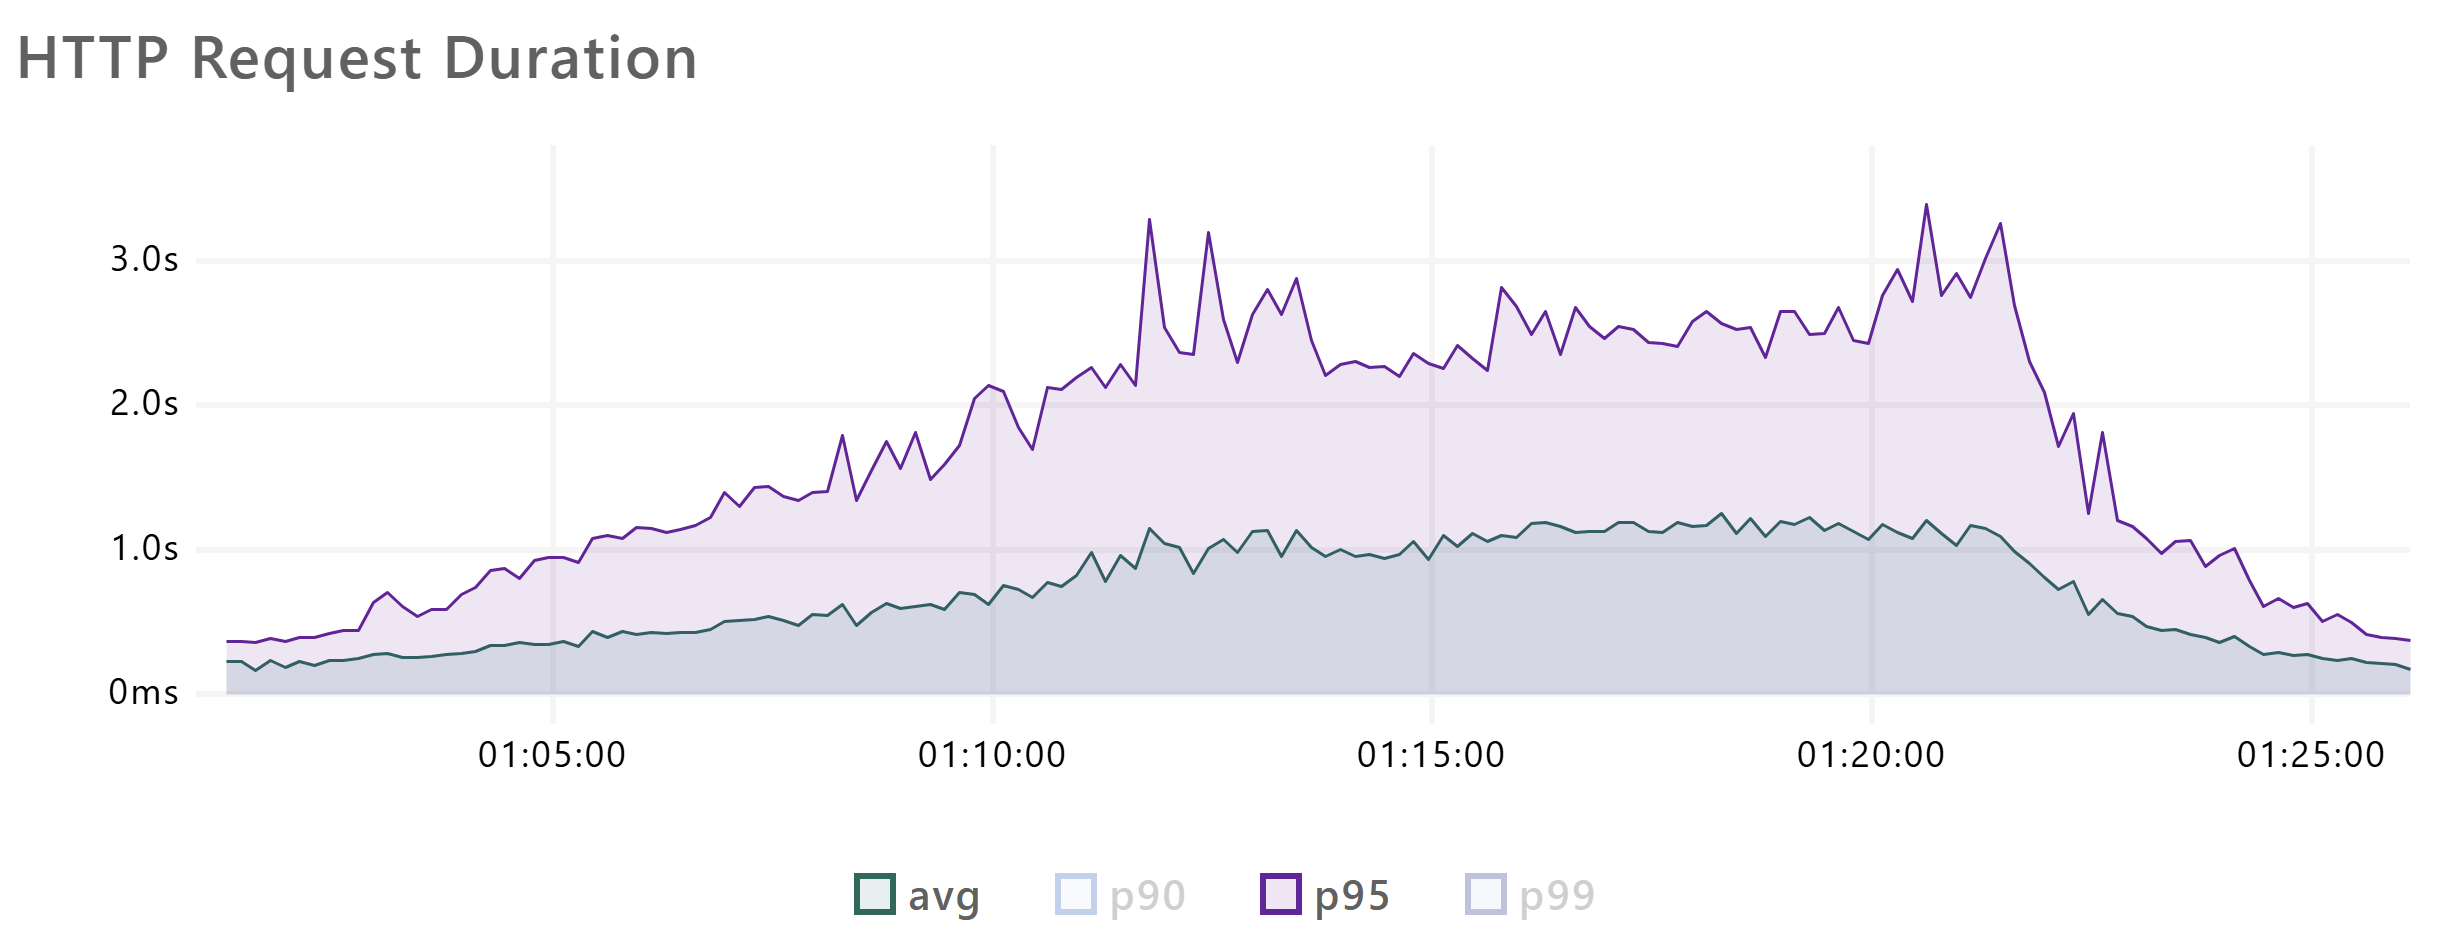
\includegraphics[width=1\textwidth]{assets/elasticity-test/req-duration.png}
    \caption{Duração das requisições ao longo do teste de elasticidade}
    \label{fig:elasticity-req-duration}
\end{figure}

A Figura \ref{fig:elasticity-req-duration} apresenta a média e o percentil 95 da duração das requisições durante o teste. A média iniciou em aproximadamente 200 ms e aumentou gradualmente à medida que o número de usuários crescia, alcançando um pico de 1,3 segundos. O percentil 95, que reflete o tempo das 5\% requisições mais lentas, chegou a um máximo de 3 segundos. Apesar do aumento na latência com a elevação da carga, os tempos de resposta permaneceram dentro de limites aceitáveis.

\begin{figure}[H]
    \centering
    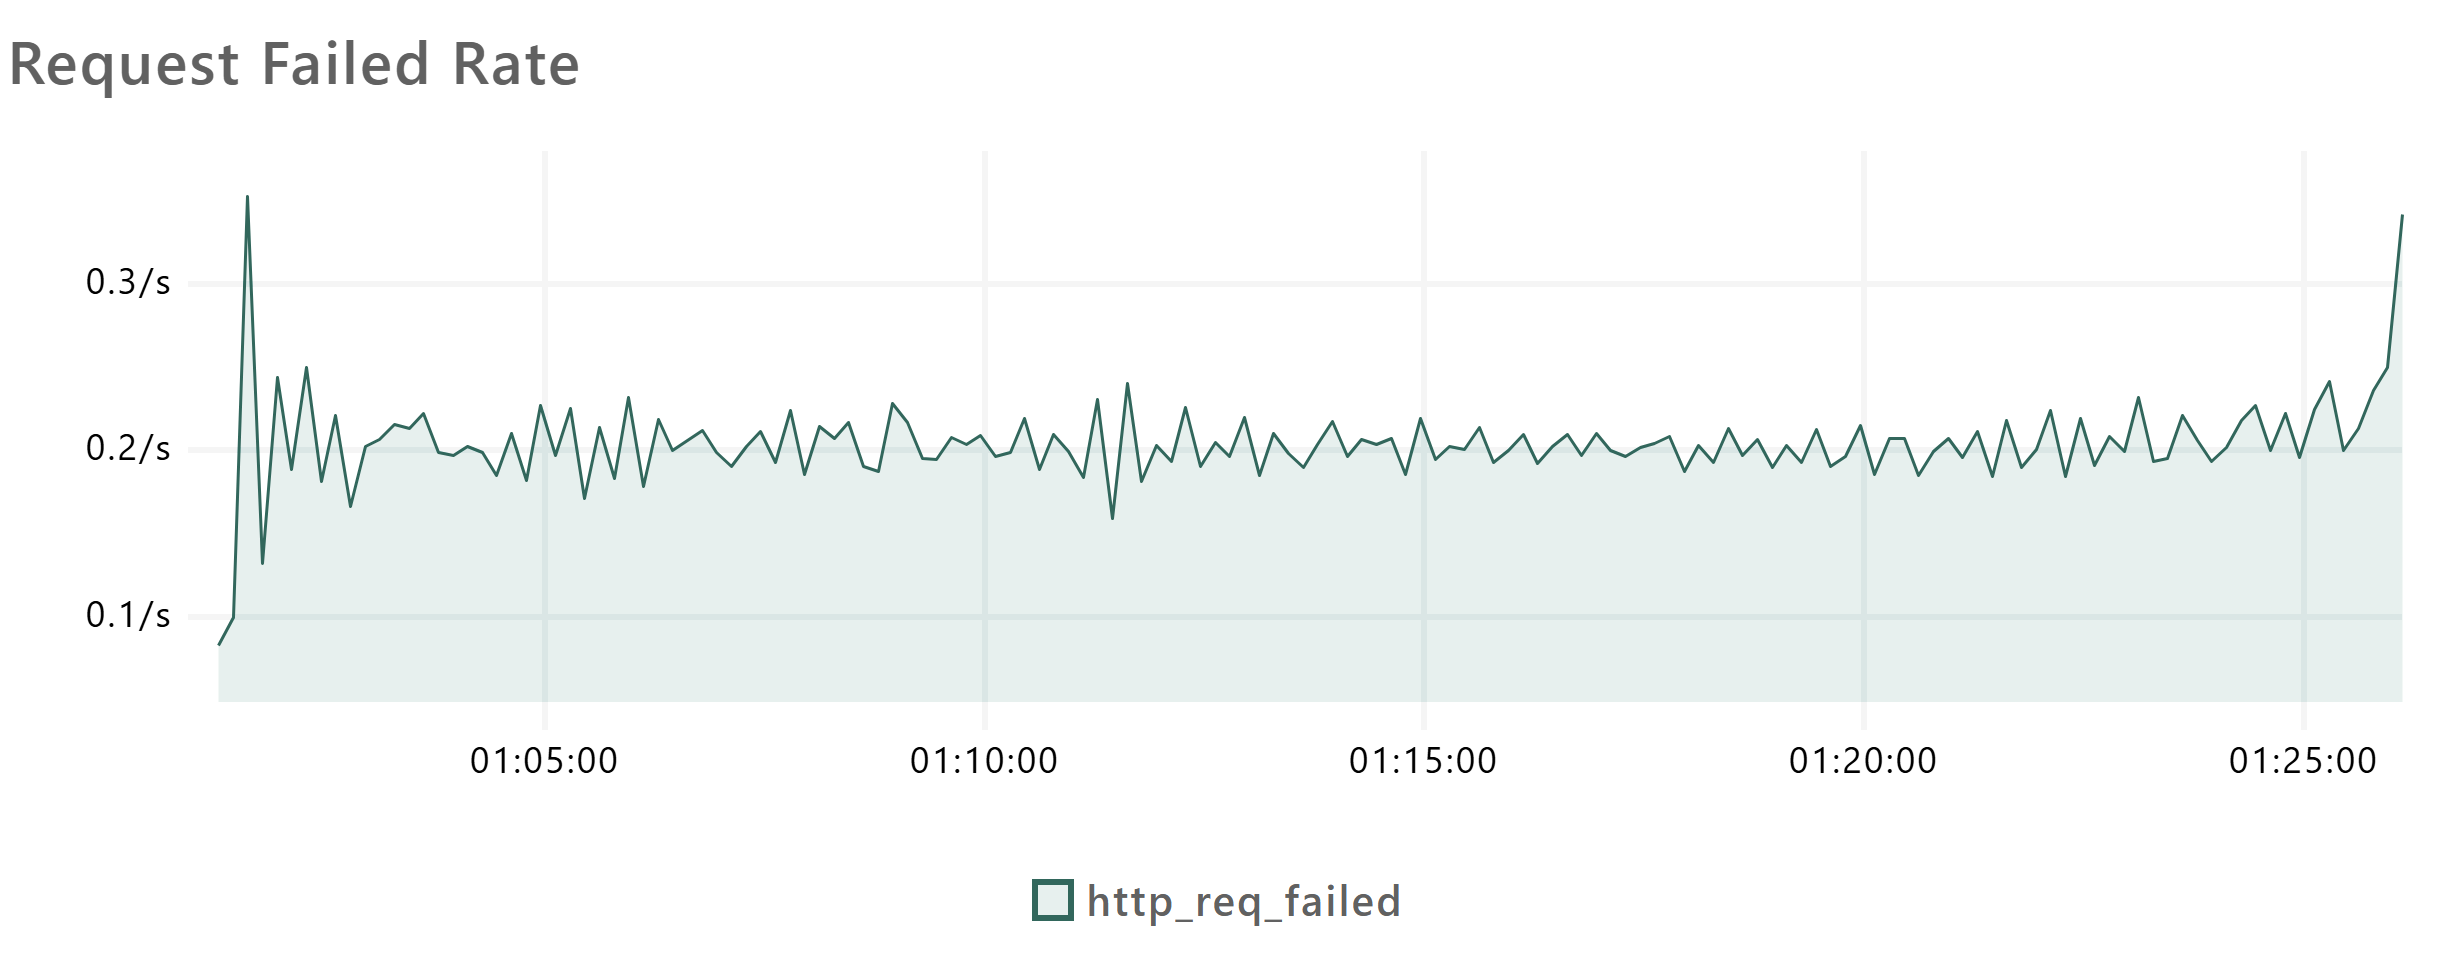
\includegraphics[width=1\textwidth]{assets/elasticity-test/req-failed-rate.png}
    \caption{Taxa de requisições falhadas ao longo do teste de elasticidade}
    \label{fig:elasticity-req-failed-rate}
\end{figure}

A taxa de requisições falhadas, ilustrada na Figura \ref{fig:elasticity-req-failed-rate}, manteve-se em torno de 0,2 requisição por segundo, representando menos de 1\% do total processado. Esses resultados evidenciam a resiliência do sistema, que lidou bem com as demandas sem falhas críticas ou interrupções significativas no serviço.

\begin{figure}[H]
    \centering
    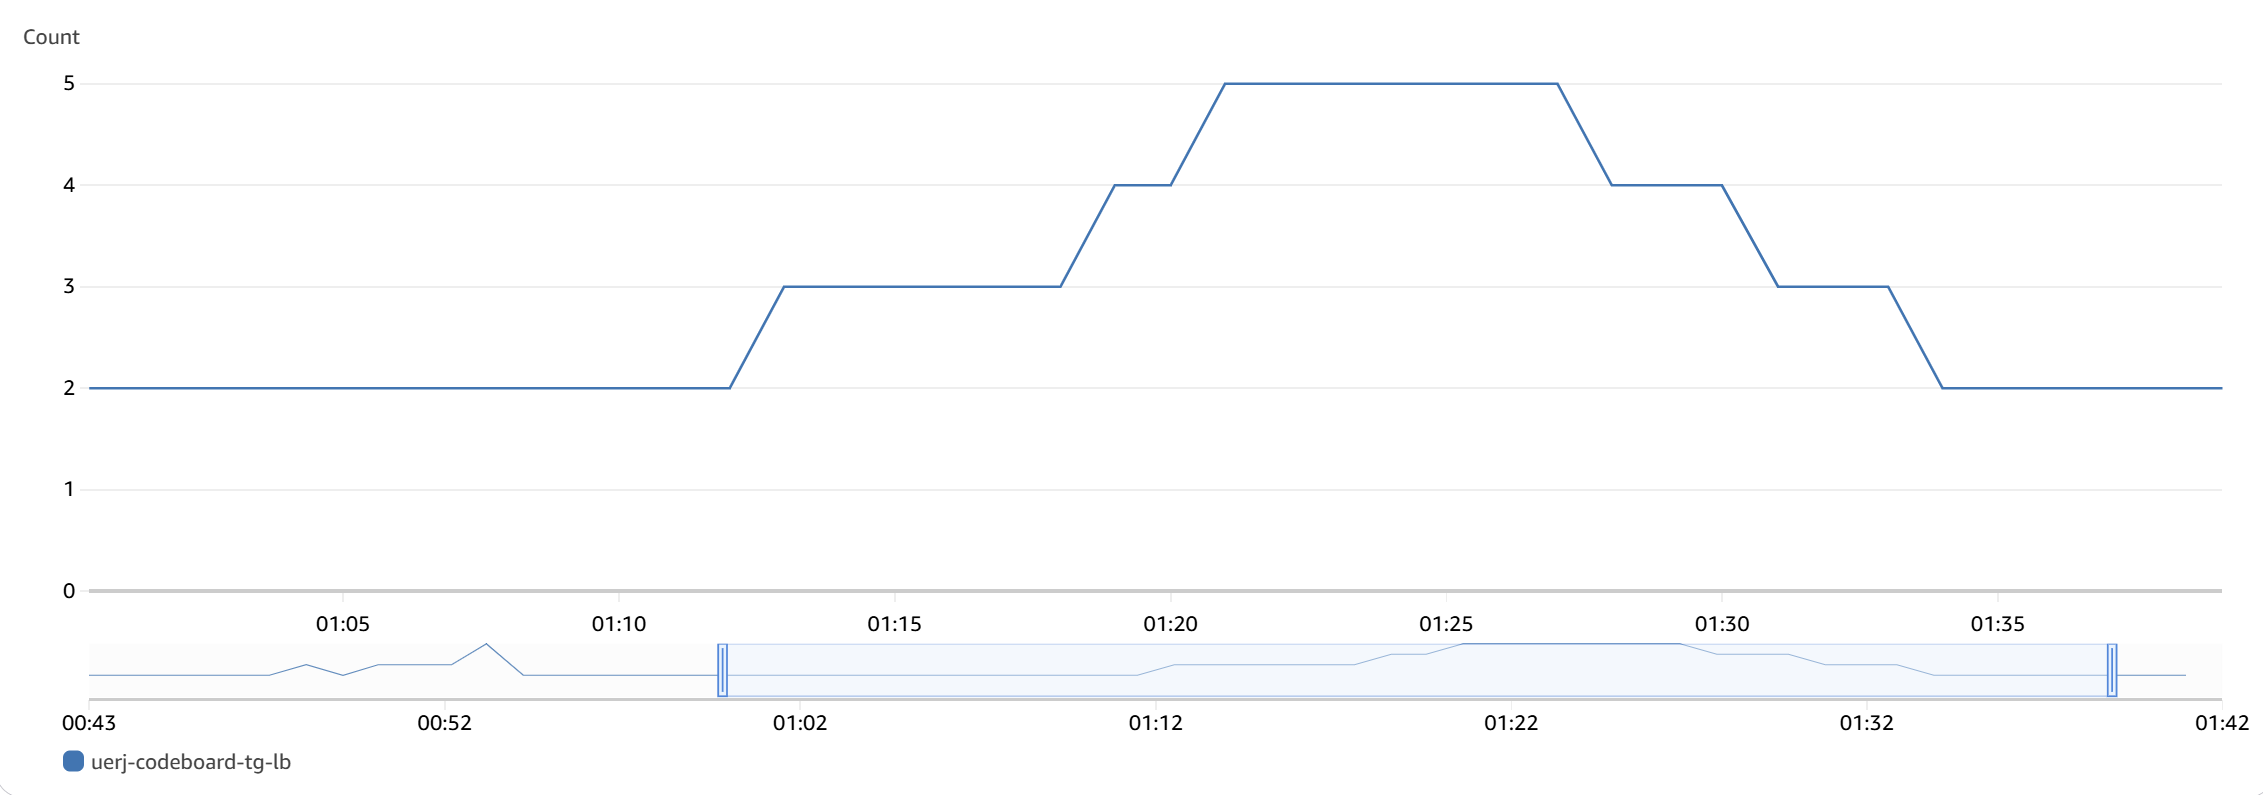
\includegraphics[width=1\textwidth]{assets/elasticity-test/healthy-hosts.png}
    \caption{Número de servidores disponíveis ao longo do teste de elasticidade}
    \label{fig:elasticity-healthy-hosts}
\end{figure}

A Figura \ref{fig:elasticity-healthy-hosts} ilustra a evolução do número de servidores disponíveis durante o teste. Nos primeiros 10 minutos, quando o número de usuários era insuficiente para impactar a infraestrutura, a quantidade de servidores permaneceu constante em dois. À medida que o número de usuários se aproximava do pico de 300, um terceiro servidor foi adicionado à infraestrutura para atender à demanda adicional. Esse padrão se repetiu conforme o crescimento do tráfego, resultando em um pico de cinco servidores. Posteriormente, com a diminuição da carga e o término do teste, os servidores adicionais foram desativados, restabelecendo o estado inicial de dois servidores. Esse comportamento demonstra a capacidade do sistema de adaptar-se dinamicamente ao tráfego, escalando horizontalmente para atender a cargas mais elevadas e reduzindo a capacidade quando a demanda diminui.

Cabe destacar que o gráfico apresentado na Figura \ref{fig:elasticity-healthy-hosts} considera apenas os servidores disponíveis para processar requisições. O tempo de inicialização de novos servidores é de aproximadamente dois minutos. Por exemplo, o gatilho para a adição de um novo servidor ocorreu por volta de 01:11, mas ele somente se tornou operacional para processar requisições em 01:13, momento em que o gráfico passou a refletir sua presença.

\begin{figure}[H]
    \centering
    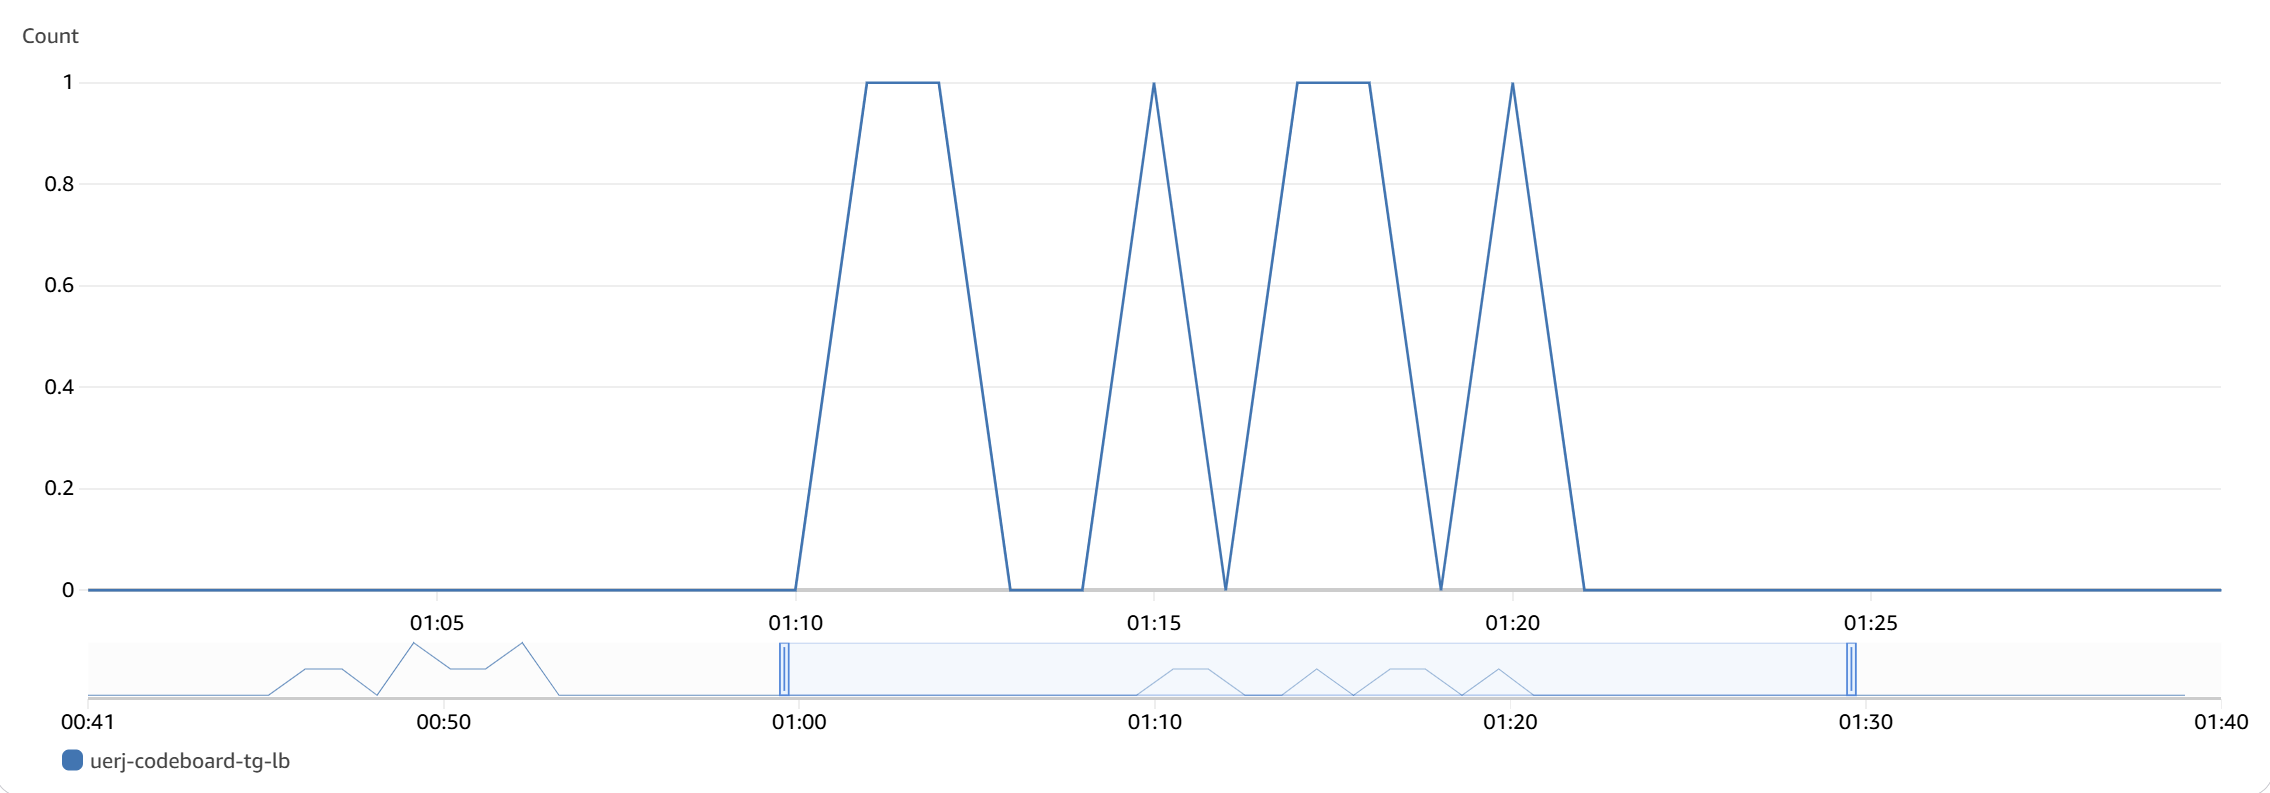
\includegraphics[width=1\textwidth]{assets/elasticity-test/unhealthy-hosts.png}
    \caption{Número de servidores não saudáveis ao longo do teste de elasticidade}
    \label{fig:elasticity-unhealthy-hosts}
\end{figure}

Por fim, a Figura \ref{fig:elasticity-unhealthy-hosts} destaca que, durante o momento de maior estresse na infraestrutura, coincidindo com a provisão de um novo servidor, um dos servidores apresentou problemas de saúde. Isso indica que o servidor estava tão sobrecarregado que não conseguia processar sequer os healthchecks, levando o balanceador de carga a marca-lo temporariamente como não saudável. No entanto, com a adição de novos servidores poucos minutos depois, o servidor conseguiu se recuperar e retornar ao processamento de requisições. Esse padrão foi observado repetidamente conforme o aumento do número de usuários, demonstrando a capacidade da infraestrutura de se adaptar dinamicamente às demandas de tráfego.


\section{Testes de Tolerância a Falhas}
% TODO: REVISAR (principalmente esse primeiro parágrafo)
% TODO: Medir o RTO

Garantir a disponibilidade da plataforma mesmo em situações de falha é essencial. Realizamos testes para verificar como a infraestrutura se comporta diante de falhas em servidores e na aplicação, e como ela se recupera desses eventos.

\subsection{Metodologia de Testes}
% TODO: Mesma do capítulo de escalabilidade, porém com valorez reduzidos e um tempo maior de manutenção da carga

Os testes de tolerância a falhas foram realizados utilizando a ferramenta Grafana K6, que permite simular um grande número de usuários acessando a plataforma simultaneamente. A ferramenta foi configurada para executar testes em diferentes estágios de carga, aumentando progressivamente o número de usuários conectados à plataforma. Dessa forma, foi possível medir o desempenho do sistema em termos de latência, taxa de erro e capacidade de resposta. Os estágios do teste foram divididos em três etapas principais:

\subsection{Falhas de Servidores}

Para simular uma falha em um servidor, foi realizado um teste de desligamento manual de um dos servidores do Brasil, com o objetivo de avaliar a capacidade da infraestrutura de se recuperar de falhas de forma automática. O desligamento foi realizado pelo painel de controle da AWS, que permite desligar um servidor de forma remota. Durante o teste, o ambiente de produção estava configurado com dois servidores e somente uma região geográfica, a do Brasil.

Durante o período de falha simulada, estavam sendo simulados 30 usuários acessando a plataforma simultaneamente da região geográfica do Brasil, a fim de avaliar o impacto da falha na disponibilidade da plataforma. Os resultados dos testes estão apresentados na Figura \ref{fig:server-failure-latency-over-time}, que traz a latência média da plataforma em relação ao tempo, sendo destacadado o momento em que ocorreu a falha no servidor, e na Figura \ref{fig:server-failure-requests-over-time}, que traz a quantidade de requisições processadas pela plataforma em relação ao tempo, sendo destacadado o momento em que ocorreu a falha no servidor. A Tabela \ref{tab:server-failure-stats} traz as estatísticas dos testes de falha em servidores, mostrando a quantidade de falhas e sucesso durante o teste.

% \begin{figure}[H]
%     \centering
%     \includegraphics[width=1\textwidth]{images/server-failure-latency-over-time.png}
%     \caption{Latência média da plataforma em relação ao tempo durante uma falha em um servidor}
%     \label{fig:server-failure-latency-over-time}
% \end{figure}

% \begin{figure}[H]
%     \centering
%     \includegraphics[width=1\textwidth]{images/server-failure-requests-over-time.png}
%     \caption{Quantidade de requisições processadas pela plataforma em relação ao tempo durante uma falha em um servidor}
%     \label{fig:server-failure-requests-over-time}
% \end{figure}

\begin{table}[H]
    \centering
    \caption{Estatísticas dos testes de falha em servidores}
    \label{tab:server-failure-stats}
    \begin{tabular}{|l|l|}
        \hline
        \textbf{Falhas}  & 0 \\ \hline
        \textbf{Sucesso} & 1 \\ \hline
    \end{tabular}
\end{table}

Como pode ser observado na Tabela \ref{tab:server-failure-stats}, a infraestrutura foi capaz de se recuperar de forma automática da falha no servidor, garantindo a disponibilidade da plataforma em situações de falha. Os gráficos da Figura \ref{fig:server-failure-latency-over-time} e Figura \ref{fig:server-failure-requests-over-time} mostram que a latência da plataforma aumentou durante o período de falha, mas retornou ao normal após a recuperação automática do servidor. Isso garante que a plataforma seja capaz de se recuperar de falhas de forma automática, garantindo a disponibilidade da plataforma em situações de falha.

Na Figura \ref{fig:server-qtty-over-time}, é possível observar a quantidade de servidores ativos em relação ao tempo, sendo destacadado o momento em que ocorreu a falha no servidor. Como pode ser observado, a infraestrutura foi capaz de se recuperar de forma automática da falha no servidor, garantindo a disponibilidade da plataforma em situações de falha.

\subsection{Falhas da Aplicação}

No teste de falhas da aplicação, foi realizado um teste de desligamento manual de um dos processos do servidor do Brasil, com o objetivo de avaliar a capacidade da infraestrutura de se recuperar de falhas de forma automática. O desligamento foi realizado por meio de um comando no terminal do servidor, utilizando uma conexão SSH e o comando kill -9 para encerrar o processo. Durante o teste, o ambiente de produção estava configurado com somente um servidor e somente uma região geográfica, a do Brasil. 

Durante o período de falha simulada, estavam sendo simulados 30 usuários acessando a plataforma simultaneamente da região geográfica do Brasil, a fim de avaliar o impacto da falha na disponibilidade da plataforma. Os resultados dos testes estão apresentados na Figura \ref{fig:process-failure-latency-over-time}, que traz a latência média da plataforma em relação ao tempo, sendo destacadado o momento em que ocorreu a falha no processo, e na Figura \ref{fig:process-failure-requests-over-time}, que traz a quantidade de requisições processadas pela plataforma em relação ao tempo, sendo destacadado o momento em que ocorreu a falha no processo. A Tabela \ref{tab:process-failure-stats} traz as estatísticas dos testes de falha em processos, mostrando a quantidade de falhas e sucesso durante o teste.

% \begin{figure}[H]
%     \centering
%     \includegraphics[width=1\textwidth]{images/process-failure-latency-over-time.png}
%     \caption{Latência média da plataforma em relação ao tempo durante uma falha em um processo}
%     \label{fig:process-failure-latency-over-time}
% \end{figure}

% \begin{figure}[H]
%     \centering
%     \includegraphics[width=1\textwidth]{images/process-failure-requests-over-time.png}
%     \caption{Quantidade de requisições processadas pela plataforma em relação ao tempo durante uma falha em um processo}
%     \label{fig:process-failure-requests-over-time}
% \end{figure}

Como pode ser observado na Tabela \ref{tab:process-failure-stats}, a infraestrutura foi capaz de se recuperar de forma automática da falha no processo, garantindo a disponibilidade da plataforma em situações de falha. Os gráficos da Figura \ref{fig:process-failure-latency-over-time} e Figura \ref{fig:process-failure-requests-over-time} mostram que a latência da plataforma aumentou durante o período de falha, mas retornou ao normal após a recuperação automática do processo. Isso garante que a plataforma seja capaz de se recuperar de falhas de forma automática, garantindo a disponibilidade da plataforma em situações de falha.

Observando os logs do servidor presentes na Figura \ref{fig:process-failure-logs}, foi possível verificar que o processo que falhou foi reiniciado automaticamente em menos de 1 segundo após a falha, garantindo a disponibilidade da plataforma em situações de falha. Isso garante que a plataforma seja capaz de se recuperar de falhas de forma automática, garantindo a disponibilidade da plataforma em situações de falha.

% \begin{figure}[H]
%     \centering
%     \includegraphics[width=1\textwidth]{images/process-failure-logs.png}
%     \caption{Logs do servidor durante uma falha em um processo}
%     \label{fig:process-failure-logs}
% \end{figure}



\section{Desempenho da Plataforma}
% TODO: Utilizar métricas do teste de elasticidade para validar o desempenho da plataforma
% TODO: VALIDAR ISSO!!!!!!!!!!!

A avaliação do desempenho da plataforma é fundamental para garantir que ela seja capaz de atender às demandas dos usuários com tempos de resposta adequados. Nesta seção, apresentamos os testes de desempenho realizados, focando em métricas como tempo de resposta geral, desempenho do Redis e desempenho do MongoDB.

\subsection{Tempo de Resposta}

Para medir o tempo de resposta da plataforma, utilizamos a ferramenta Grafana K6 para simular múltiplos usuários acessando várias funcionalidades da aplicação, como login, criação de salas e edição de código. Foram realizadas simulações com quantidades crescentes de usuários simultâneos, variando de 100 a 1000 usuários.

Os resultados mostraram que, com até 500 usuários simultâneos, o tempo médio de resposta permaneceu abaixo de 200 ms, considerado adequado para uma aplicação web interativa. Ao exceder 800 usuários simultâneos, observou-se um aumento significativo na latência, chegando a tempos de resposta médios de 500 ms. Esses resultados indicam a necessidade de ajustes na infraestrutura ou de uma escalabilidade horizontal para atender a cargas mais elevadas.

\section{Testes de Segurança}
% TODO: VALIDAR

A segurança é um aspecto crítico em qualquer aplicação web. Nesta seção, apresentamos os testes de segurança realizados para identificar vulnerabilidades e assegurar a proteção dos dados dos usuários.

\subsection{Testes de Firewall}

Realizamos varreduras de portas e tentativas de acesso não autorizado para verificar se os firewalls estão corretamente configurados. Utilizamos ferramentas como o Nmap para identificar portas abertas e simular ataques.

% TODO: Inserir resultados dos testes de firewall

Os testes confirmaram que apenas as portas essenciais estão abertas (por exemplo, portas 80/443 para HTTP/HTTPS), e que existem regras de firewall bloqueando tentativas de acesso não autorizado. Isso sugere que o firewall está configurado de forma adequada.

\subsection{Criptografia}

Verificamos a utilização de criptografia nas comunicações, garantindo que todo o tráfego entre o cliente e o servidor seja seguro. Utilizamos ferramentas como o SSL Labs para analisar o certificado SSL/TLS e as configurações de segurança.

Os resultados mostraram que a plataforma utiliza certificados válidos e protocolos seguros (TLS 1.2 ou superior), com preferência por conjuntos de cifras fortes. Isso diminui o risco de interceptação ou ataque man-in-the-middle.


\section{Testes de Monitoramento}
% TODO: VALIDAR

O monitoramento contínuo da infraestrutura é fundamental para a detecção prévia de problemas e para a manutenção da disponibilidade e desempenho da plataforma de forma proativa. Nesta seção, apresentamos os testes de monitoramento realizados na plataforma Codeboard UERJ.

\subsection{Monitoramento de Recursos}
% TODO: precisa mesmo?

Utilizando o CloudWatch, monitoramos os recursos da infraestrutura, como CPU, memória, tráfego de rede e armazenamento. Configuramos alarmes para notificar a equipe de operações em caso de uso excessivo ou falhas nos recursos.

Os dashboards configurados permitem visualizar em tempo real o estado da infraestrutura e identificar tendências ou anomalias. Durante os testes de carga, foi possível observar o comportamento dos recursos e tomar decisões informadas sobre a necessidade de escalonamento.

\subsection{Alertas de Incidentes}

Configuramos sistemas de alerta que notificam a equipe de operações em caso de incidentes, como alta latência, aumento na taxa de erros ou indisponibilidade de servidores. As notificações são enviadas via e-mail e mensagens instantâneas, permitindo resposta rápida.

Durante os testes de falha, os alertas foram acionados conforme esperado, comprovando a eficácia do sistema de monitoramento e notificações.

